\subsection{Illustrative Example}
We note there are problems one can formulate where the observed density corresponds directly to a normalized likelihood function familiar to Bayesian statisticians, as we demonstrate below.
One difference between $\updated$ and $\posterior$ is the use of normalizing constant $C$ in $\posterior$ not present in $\updated$, which has a function in its denominator .
The property of $\updated$ that allows this is explained by Corollary~\ref{cor:int} below.
To illustrate the differences in the two densities, we first explore the impact of this difference in the example below, taken from \cite{BJW18}.

%%%%%


\begin{ex}
Suppose $\pspace = [-1,1]\subset\RR$ and $Q(\param)=\param^5$ so that $\dspace = [-1,1]$.
For the observation-consistent framework, we assume $\initial\sim \mathcal{U}([-1,1])$ and $\observed\sim N(0.25,0.1^2)$.
The push-forward of initial PDF, the observed PDF, and the updated PDF are shown in Fig.~\ref{fig:bayes-comparison}.

For the Bayesian inverse problem, we assume $d\in \dspace$ with $d=Q(\paramref)+\xi$ where $\xi\sim N(0,0.1^2)$.
%In particular, we assume that $d=0.25$ and follow the process of \cite{Stuart_Bayesian} to form the data-likelihood function so that it matches the observed density.
We then construct $\pi_{\text{post}}(\param \, |\, d)$ for this example assuming a uniform prior (to match the initial density) with an assumed observed value of $d=0.25$ so that the data-likelihood function matches the observed density.
The posterior and its push-forward are also shown in Fig.~\ref{fig:bayes-comparison}.

While the updated and posterior densities in Fig.~\ref{fig:bayes-comparison} share certain similarities (e.g., they are uni-modal with similar locations of the mode), they are otherwise visibly distinct.
The differences between these densities is made more evident by examining their push-forwards.
The push-forward of the updated density agrees well with the observed density, which is to be expected.
However, the push-forward of the posterior is bi-modal and does not match the observed density, which we recall is identical to the data-likelihood function in this case.
%with peaks that appear to align fairly well with the two distinct peaks of the predicted density and observed density.
%Recall that the observed density and data-likelihood are, in this case, identical.
%Moreover, with the setup described above, the predicted density can also be interpreted as the push-forward of the prior density.
%This demonstrates the regularizing impact of the prior on the posterior and how i.

%
%Hierarchical Bayesian methods \cite{} extend this typical framework to problems where aleatoric uncertainties are present, but are still fundamentally developed from a  point estimation perspective.
%Specifically, prior distributions are specified from a parametric family of distributions, such as Gaussian distributions, and the hyper-parameters used to define that family of distributions, such as the means and variances, become a focal point of estimation by the methodology.


\begin{figure}[htbp]
\centering
   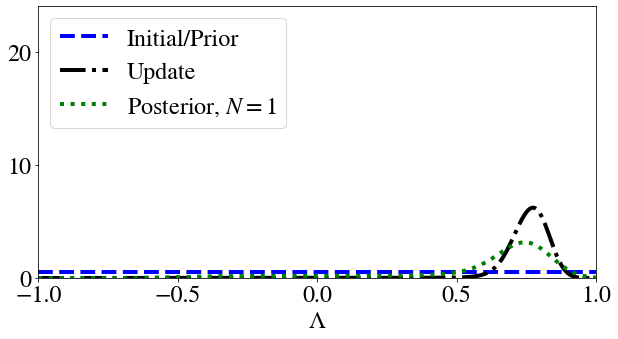
\includegraphics[width=0.49\linewidth]{figures/bip-vs-sip-1.png}
   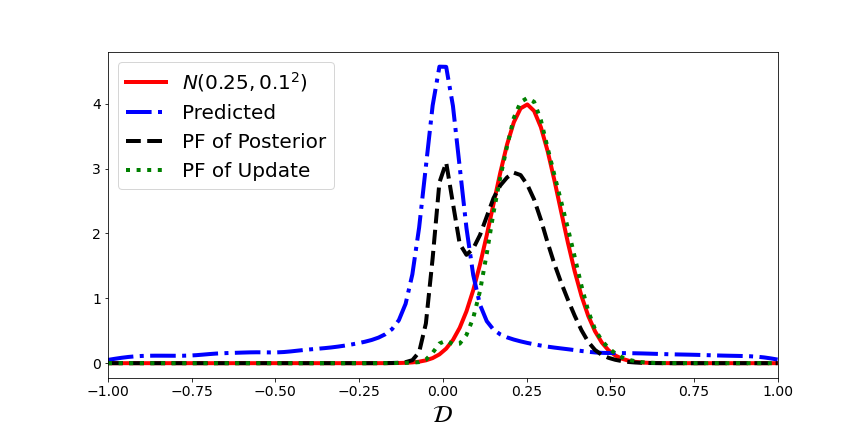
\includegraphics[width=0.49\linewidth]{figures/bip-vs-sip-pf-1.png}
 \caption{(Left) The initial/prior PDF $\initial$ (blue solid curve), updated PDF $\updated$ (black dashed curve), and posterior PDF $\pi_\text{post}$ (green dashed-dotted curve) on $\Lambda$.
 (Right) The push-forward (PF) of the initial/prior PDF $\predicted$ (blue solid curve), observed/likelihood PDF (red solid curve), PF of the updated PDF $\updated$ (black dashed curve), and the PF of the posterior PDF $\pi_\text{post}$ (green dashed-dotted curve) for the QoI.}
 \label{fig:bayes-comparison}
\end{figure}

The takeaway to the above discussion and example is that each density is solving a {\em different} inverse problem.
The posterior density is intended to provide point estimates of a true parameter value whereas the updated density is intended to quantitatively characterize natural variations in parameter values.

\end{ex}

\begin{ex}
We reformulated the previous example to make the role of data collection more central.
Specifically, suppose $Q(\paramref)=0.25$ and noisy measurement data are drawn from a $N(0.25,0.1^2)$, i.e., we assume that $d=Q(\paramref)+\xi$ where $\xi\sim N(0,0.1^2)$.
For the SIP, we could use the sample mean and variance of this data to estimate the ``exact'' observed $N(0.25,0.1^2)$ distribution whereas the data-likelihood would involve a product of normal densities.
We draw $S=5, 10, \text{ and}, 20$ samples to form the estimate of the mean and the likelihood function, and show the results in Figure~\ref{fig:bayes-comparison-convergence}
In this case, the objective is to use the posterior or updated density to produce an estimate of $\paramref$.

\begin{figure}[htbp]
\centering
   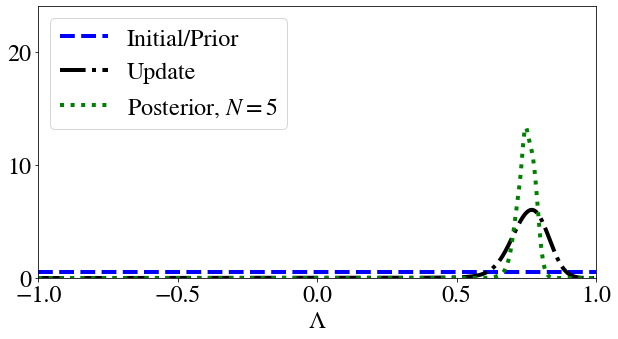
\includegraphics[width=0.49\linewidth]{figures/bip-vs-sip-5.png}
   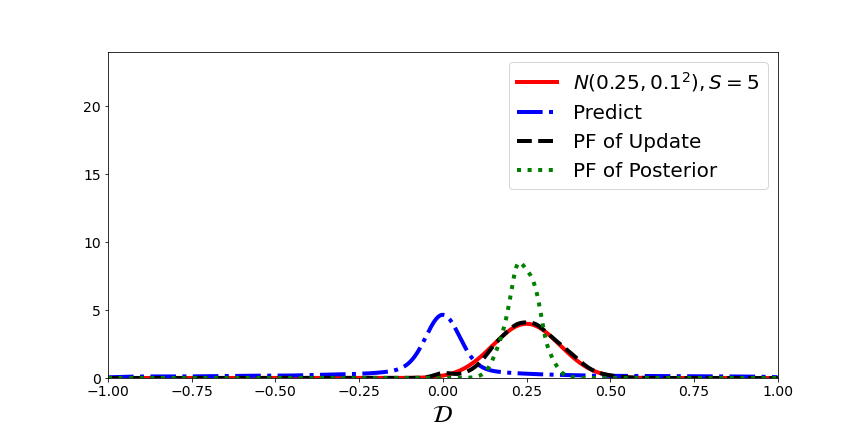
\includegraphics[width=0.49\linewidth]{figures/bip-vs-sip-pf-5.png}
   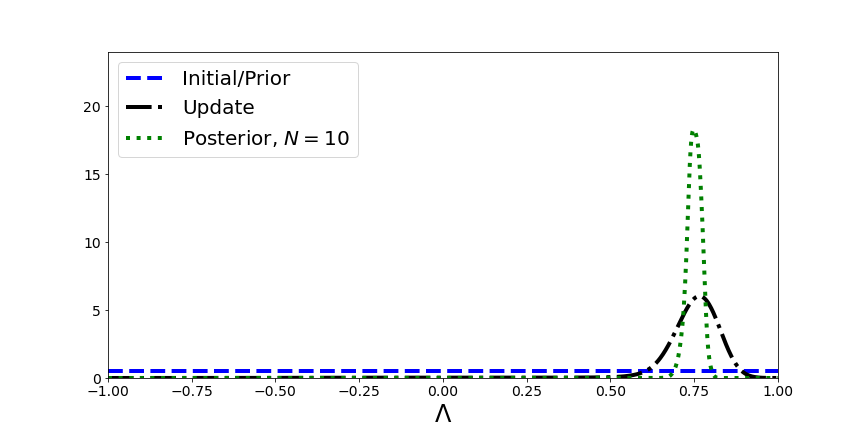
\includegraphics[width=0.49\linewidth]{figures/bip-vs-sip-10.png}
   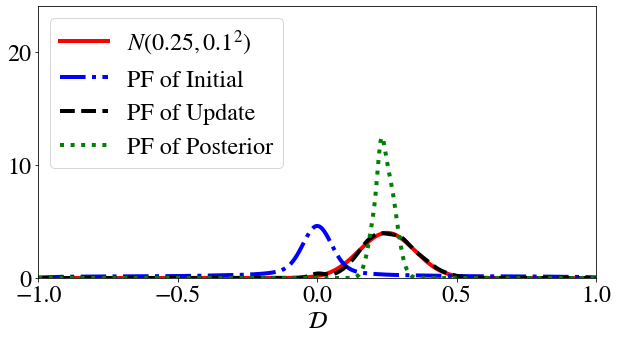
\includegraphics[width=0.49\linewidth]{figures/bip-vs-sip-pf-10.png}
   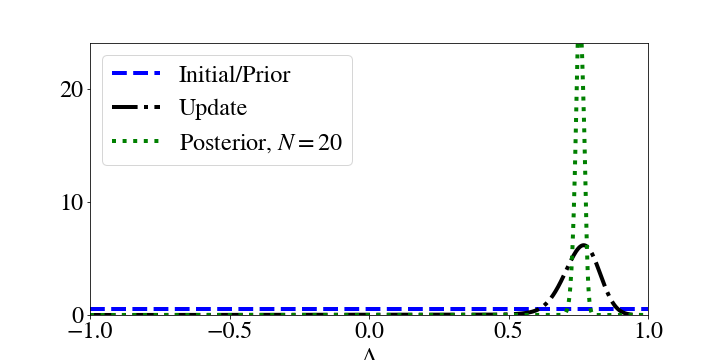
\includegraphics[width=0.49\linewidth]{figures/bip-vs-sip-20.png}
   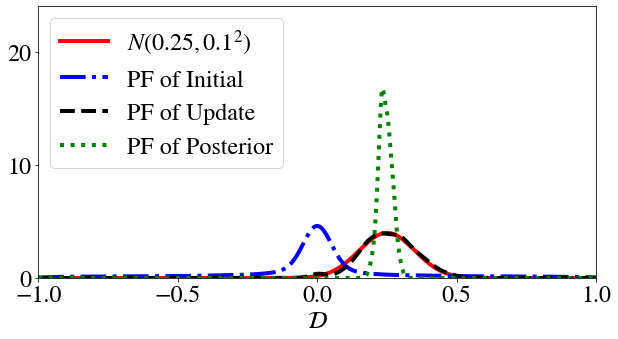
\includegraphics[width=0.49\linewidth]{figures/bip-vs-sip-pf-20.png}
 \caption{(Top to Bottom): $S=5, 10, \text{ and}, 20$ samples are used to solve the SIP and BIP for comparison. (Left) The initial/prior PDF $\initial$ (blue solid curve), updated PDF $\updated$ (black dashed curve), and posterior PDF $\pi_\text{post}$ (green dashed-dotted curve) on $\Lambda$.
 (Right) The push-forward (PF) of the initial/prior PDF $\predicted$ (blue solid curve), observed/likelihood PDF (red solid curve), PF of the updated PDF $\updated$ (black dashed curve), and the PF of the posterior PDF $\pi_\text{post}$ (green dashed-dotted curve) for the QoI.}
 \label{fig:bayes-comparison-convergence}
\end{figure}

We find that the updated distribution becomes more centered around the true parameter value $\paramref$, but the uncertainty in the estimate does not change.
By contrast, the posterior increases in confidence alongside the likelihood function.
This further illustrates the point made earlier: the BIP and SIP are solving fundamentally different problems (they are addressing different questions).
As more data is incorporated, the goal of the BIP is to reduce epistemic uncertainty; for the SIP, it is aleotoric.
\end{ex}




%%%%%

In summary, it is not the goal of Bayesian inference to construct a pullback distribution.
Bayesian inverse problems are fundamentally posed as parameter-identification, not distribution estimation.
However, one could assume that a posterior on $\pspace$ can be expressed as a Gaussian distribution, and solve for the most likely mean and standard deviation that characterizes it [TK - cite more] \cite{Smith}.
This defines what is commonly referred to a as a Hierarchical Bayesian Inverse Problem.
More complex densities can be approximated by mixture models.

For example, one can assume that the posterior can be given by a linear combination of four Gaussian distributions, and solve for eight parameter values (four standard deviations and means).
However, the operative word here is \emph{assume}; in order to capture a density using a Bayesian framework, one needs to impose some sort of explicit structure on the posterior.
No such compromise is required in the Data-Consistent Inversion framework.
Distributions (or measures) can be solved for directly, regardless of any nonlinear/non-parameteric structure by leveraging the measure-theoretic approach described in \cite{BE13} or \cite{BJW18}.

The Hierarchical Bayesian inverse problem casts a distribution-estimation problem in the context of parameter identification.
As a complementary line of reasoning, one can ask what it means to cast a parameter identification problem in a distribution-estimation context.
In the next chapter, we motivate the use of the maximal updated density point (maximizing the update), as a means of providing a useful point estimate to parameters.
Before making this connection, we must establish that the framework in which such a question is asked is rigorously defined.
In the next section, we finish presenting the Data-Consistent Framework by summarizing key results about the stability and numerical convergence of the updated solution \eqref{eq:updated-pdf} to the SIP.

\FloatBarrier
